\chapter{Introdução}
\label{sec:introducao}

    Este capítulo tem como objetivo apresentar o contexto, a motivação, a metodologia, os problemas que este trabalho visa abordar, bem como a organização do texto.

    \section{Contextualização}

    Com o avanço da digitalização, o desenvolvimento de software tornou-se uma atividade fundamental no contexto contemporâneo, no qual as organizações buscam evoluir digitalmente para garantir sua competitividade no mercado \cite[]{cardoso2019and}. Em decorrência disso, o prazo para a entrega de sistemas tem se reduzido progressivamente, o que pode resultar em práticas de desenvolvimento inadequadas, comprometendo a qualidade do software \cite[]{Kuutila2019Time}. Nesse contexto, boas práticas tornam-se fundamentais para manter um projeto de qualidade, o que facilita sua escalabilidade e manutenção.

    As boas práticas de desenvolvimento de software consistem em técnicas utilizadas antes e durante  a fase de desenvolvimento, visando garantir a qualidade, escalabilidade, manutenibilidade e segurança \cite[]{braga2007visao}. Alguns padrões utilizados na indústria de sistemas da informação é o versionamento de código com git, testes automatizados, criação de códigos genéricos para reutilizar, documentação clara, padrões de design e projeto, revisão de código, criação de diagramas da UML e planejamento de arquitetura bem detalhada. Embora haja a presença dessas boas práticas, nem todo processo de desenvolvimento de um software utiliza, como ocorre em projetos que são realizados de forma apressada, sem um processo definido ou padronização, os quais são chamados de \textit{Go Horse} \cite[]{sturmaplicaccao} pela comunidade de desenvolvedores.

    O termo \textit{Go Horse} surgiu de maneira informal e humoristica no cenários do desenvolvimento de software. Essa expressão, principalmente no Brasil, descreve projetos que foram conduzidos de forma improvisada, sem um planejamento prévio adequado, testes e documentações. Essa má prática, prioriza entregas rápidas, entretanto com pouca qualidade, resultando assim em falhas no sistema, difícil manutenção e elevados riscos para falhas de segurança, indo contra os padrões de metodologias ágeis \cite[]{perry2016funccao}.

    O projeto Web Gerenciador para Instituicões Assistenciais (WeGIA) foi desenvolvido por alunos do curso técnico do CEFET-RJ - campus Nova Friburgo. Sua criação surgiu pela falta de softwares \textit{Open Sources}, cujo seu objetivo central é melhorar a gestão, controle e transparência das entidades publicas. Sua versão atual possui seis módulos, sendo eles: o de contribuição e sócios, material e patrimônio, memorando, pessoas, pet e saúde \cite[]{latinoware2024wegia}. Apesar da relevância do projeto, este foi elaborado sem a observância de boas práticas, além de ter sido desenvolvido por alunos frequentemente sem experiência anterior e aprendendo durante o processo, o que acarretou um código com manutenção complexa, dificuldades para evolução e algumas vulnerabilidades.

    O intuito deste trabalho é a refatoração do WeGIA, que apresenta traços característicos de um projeto com abordagem \textit{Go Horse}, e servirá como fundamento para o estudo e a prática de boas práticas de desenvolvimento.

    \section{Problemas investigados}

    Projetos conduzidos sob a abordagem \textit{Go Horse} tendem a garantir sistemas que envelhecem rapidamente, tornando-se mais difícil de manter sua atualização e manutenção gradual. Esse fenômeno acaba gerando diversas soluções improvisadas durante o desenvolvimento \cite[]{oliveira2019investigaccao}. Aliada à falta de documentação, esses sistemas acabam se tornando rígidos, gerando um grau de complexidade elevado para a entrada de novos desenvolvedores na equipe e aumentando o risco de falhas a cada modificação realizada.

    Embora não seja um conceito formal na literatura acadêmica,  \textit{Go Horse} se relaciona com problemas amplamente discutidos nos dias atuais, como \textbf{dívida técnica}, \textbf{antipadrões de software}, \textbf{código legado} e \textbf{ad hoc} \cite[]{dantas2002suporte, de2021identificaccao}. Compreender o impacto no desenvolvimento de software evidencia a necessidade de aplicar boas práticas de desenvolvimento, garantindo que um projeto improvisado se transforme em um sistema sustentável e de fácil manutenção.

    O Wegia apresenta diversas características de um projeto com dívidas técnicas adquiridas no decorrer do tempo, tais como a falta de testes automatizados, tabelas sem normalização, código sem padrões estabelecidos, baixa segurança, documentação incompleta e uma arquitetura rígida. Essas características acabam impactando em retrabalho, demostivação da equipe e insatisfação de pessoas envolvidas \cite[]{borges2022investigaccao}

    Por estar no mercado de código livre, considera-se que novos usuario irão se utilizar e dar melhorias no projeto. Com isso, torna-se primordial a existencia de uma documentação clara e padrões de códigos pré estabelicidos, permitindo que o conhecimento sobre o software seja passada de forma fácil e prática entre membros da comunidade que se interessem pelo projeto.\cite[]{souza2010contribuiccao}

    Diante esse cenário e os problemas investigados, surge a questão de pesquisa desse trabalho: \textbf{Quais técnicas e boas práticas de desenvolvimento de software podem ser empregadas na refatoração de sistemas legados para garantir segurança, escalabilidade e facilidade de manutenção?}

    \section{Objetivos}
    \label{subsec:objetivos}

    Em face das dificuldades relacionadas ao desenvolvimento \textit{Go Horse}, a refatoração de um software que utiliza tecnologias obsoletas e práticas inadequadas aparece como uma abordagem estratégica. Portanto, o objetivo geral do presente trabalho consiste em refatorar o sistema, implementando boas práticas de programação, a fim de evitar o seu desgaste. Esse objetivo central pode ser subdividido em objetivos específicos, tais como:

    \begin{itemize}
        \item Reorganizar a aplicação, efetuando a transição de um sistema legado para uma arquitetura atual, empregando tecnologias atuais e amplamente utilizadas no mercado.
        \item Demonstrar o passo a passo da refatoração de um projeto legado, evidenciando as dificuldades encontradas e as soluções adotadas;
        \item Validar a melhoria da qualidadeda aplicação após sua migração tecnológica.
    \end{itemize}


    \section{Metodologia}

    % Design Science Research precisa ser um processo baseado em eviadencias, ou seja, cada etapa gera um artefato que normalemnte serve como entrada para a proxima etapa. Além disso, é bem classico o uso de ciclos iterativos, onde a cada ciclo uma nova versao do artefato eh gerada e avaliada. Favor revisar a metodologia para melhorar o processo. Podemos falar em call
    Este trabalho se inspirou no modelo \textit{Design Science Research} \cite[]{pimentel2020dsr}, sendo adaptado conforme as necessidades específicas do projeto conforme ilustrado na Figura~\ref{fig:metodologia_utilizada}.:

    \begin{figure}[H]
        \centering
        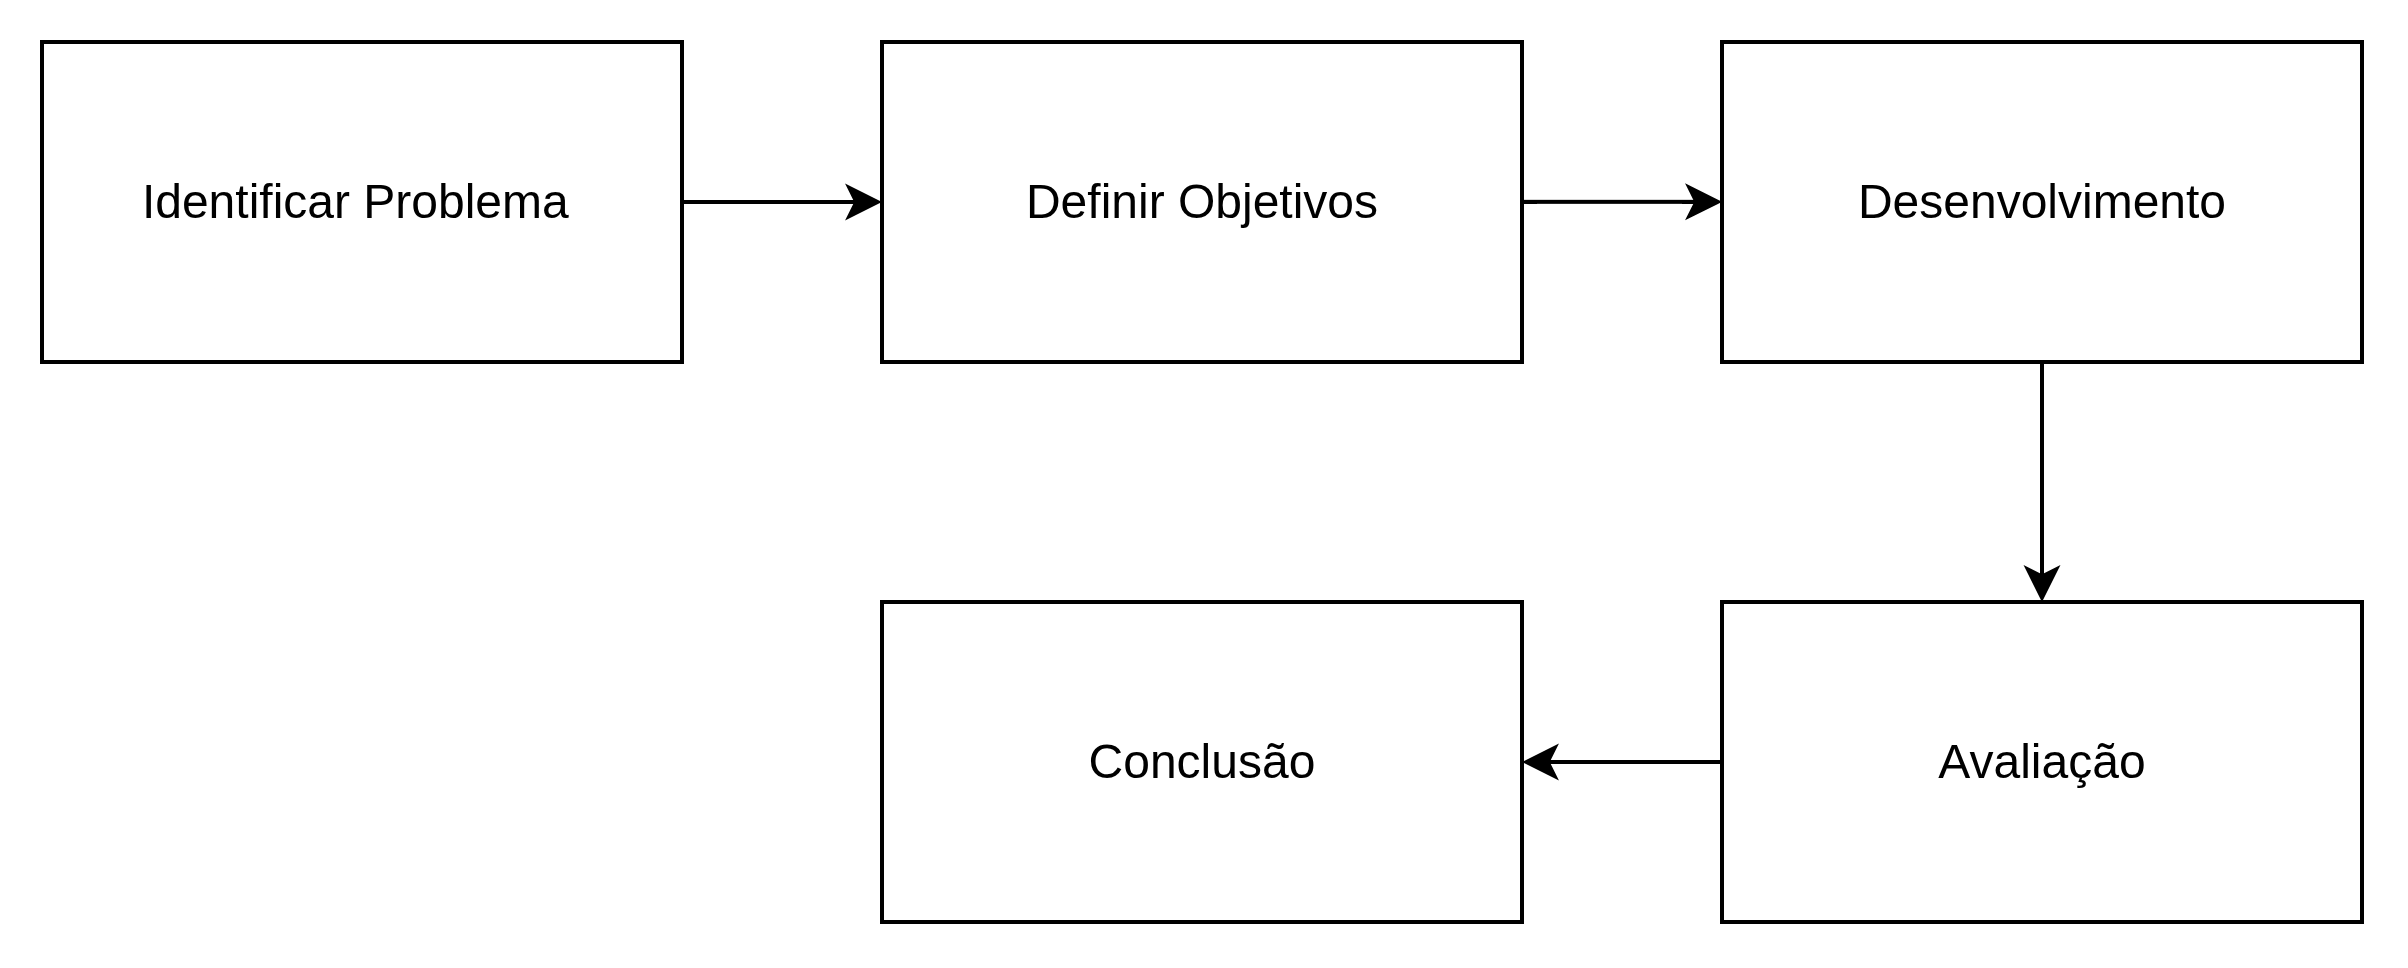
\includegraphics[width=1\linewidth]{imagens/Metodologia_utilizada.png}
        \caption{Fluxo metodológico utilizado e adaptado \citep{pimentel2020dsr} .}
        \label{fig:metodologia_utilizada}
    \end{figure}

     \begin{itemize}
        \item \textbf{Identificar Problema}:
            Nesta Etapa, realizou-se uma analisada no atual código fonte do projeto do WeGIA e no seu banco de dados para buscar informações do que poderia ser melhorado. Além disso, teve um estudo conforme o artigo \cite[]{latinoware2024wegia} onde ocorreu uma pesquisa de campo para uma análise mais aprofundada das necessidades dos usuários no sistema.
        \item \textbf{Definir Objetivos}:
            Esta etapa segue os objetivos citados dentro da introdução na subseção \ref{subsec:objetivos}, os quais orientaram a reconstrução do sistema na etapa de desenvolvimento. Para que fosse possível alcançar esse objetivo, foram utilizadas as tecnologias Laravel no backend e Nuxt.js no frontend, adotando padrões de arquitetura REST.
        \item \textbf{Desenvolvimento}:
            Nessa etapa, foi realizada a migração tecnológica visando buscar um sistema com uma arquitetura modular, escalável, seguro e moderno.
        \item \textbf{Avaliação}:
            O sistema após a reconstrução, foi submetido a diversos testes, como de carga e manuais, garantindo que todas suas funcionalidades estejam de acordo com o planejado.
        \item \textbf{Conclusão}:
            Os resultados obtidos na etapa de avaliação foi utilizada para revisar a solução proposta e identificar oportunidades de melhorias em cima dela.
    \end{itemize}

    \section{Organização do texto}

    Este projeto de conclusão de curso está dividio em cinco capítulos. O atual introduziu e contextualizou sobre o assunto abordado, evidenciando os problemas investigados e a questão de pesquisa

    O capítulo 2 aborda a  fundamentação teorica sobre o tema, servindo como  base para entendimentos dos demais capítulos.

    O Capítulo 3 apresenta os trabalhos relacionados, discutindo estudos anteriores sobre o tema de reestrutração de software.

    O Capítulo 4 descreve a proposta de solução do trabalho, apresentando caraterísticas, diagramação, tecnicas utilizadas, testes realizados e avalições descrito em mais detalhes.

    O capítulo 5 conclui o trabalho, apresentando uma discussão final sobre o tema, bem como sugestões de trabalhos futuros e considerações finais.
